\clearpage
\section{典型例题与动态响应分析}
\label{sec:ch3-worked-examples}

\noindent 动态测量问题可从三个方面展开：计算给定输入的稳态响应，由允许误差选择装置参数，以及比较参数变化对测量结果的影响。以下采用 $\omega=2\pi f$，系统相位差为“输出相位减输入相位”；$A(\omega)$ 表示幅值比，归一化后静态增益取1。\textbf{稳态输出不含随时间衰减的启动暂态。}

\subsection{例题1：多频信号通过一阶装置的稳态响应}
\keypoint{复习重点：按频率分别乘幅值比、加系统相位，再利用叠加性相加。}

\qs{双频余弦的稳态输出}{求周期信号
\[
x(t)=0.5\cos(10t)+0.2\cos(100t-45^\circ)
\]
通过传递函数 $H(s)=1/(0.005s+1)$ 的装置后的稳态响应，并分析不同频率成分的幅值、相位变化。
}

\sol
\textbf{先识别角频率，不把 $10$ 与 $100$ 当作Hz。}
本题 $K=1$、$\tau=0.005\,\mathrm{s}$，两成分的角频率为
$\omega_1=10\,\mathrm{rad/s}$、$\omega_2=100\,\mathrm{rad/s}$，分别对应约 $1.592$、$15.915\,\mathrm{Hz}$。频响为
\[
H(\iu\omega)=\frac{1}{1+\iu0.005\omega},\quad
A(\omega)=\frac{1}{\sqrt{1+(0.005\omega)^2}},\quad
\phi(\omega)=-\arctan(0.005\omega).
\]

对第一项，$\omega_1\tau=0.05$，因此
\[
A_1=\frac{1}{\sqrt{1+0.05^2}}=0.998752,\quad
\phi_1=-\arctan0.05=-2.8624^\circ,
\]
\[
y_1(t)=0.5A_1\cos(10t+\phi_1)
\approx0.499376\cos(10t-2.8624^\circ).
\]
对第二项，$\omega_2\tau=0.5$，因此
\[
A_2=\frac{1}{\sqrt{1+0.5^2}}=0.894427,\quad
\phi_2=-\arctan0.5=-26.5651^\circ.
\]
\textbf{保留原相位 $-45^\circ$，再加上装置引起的滞后：}
\[
y_2(t)=0.2A_2\cos(100t-45^\circ+\phi_2)
\approx0.178885\cos(100t-71.5651^\circ).
\]
由线性叠加性，
\[
\boxed{\begin{aligned}
y_{\mathrm{ss}}(t)\approx{}&0.499376\cos(10t-2.8624^\circ)\\
&+0.178885\cos(100t-71.5651^\circ).
\end{aligned}}
\]
上式的常相位用角度标注；数值计算时，应将其换算为弧度，与 $\omega t$ 保持一致。

\begin{table}[H]
\centering\small
\begin{tabular}{@{}c c c c c@{}}
\toprule
$\omega$（$\mathrm{rad/s}$） & 输入幅值 & 输出幅值 & 振幅衰减 & 系统相位差 \\
\midrule
$10$ & $0.5$ & $0.499376$ & $0.1248\%$ & $-2.8624^\circ$ \\
$100$ & $0.2$ & $0.178885$ & $10.5573\%$ & $-26.5651^\circ$ \\
\bottomrule
\end{tabular}
\end{table}

\begin{center}
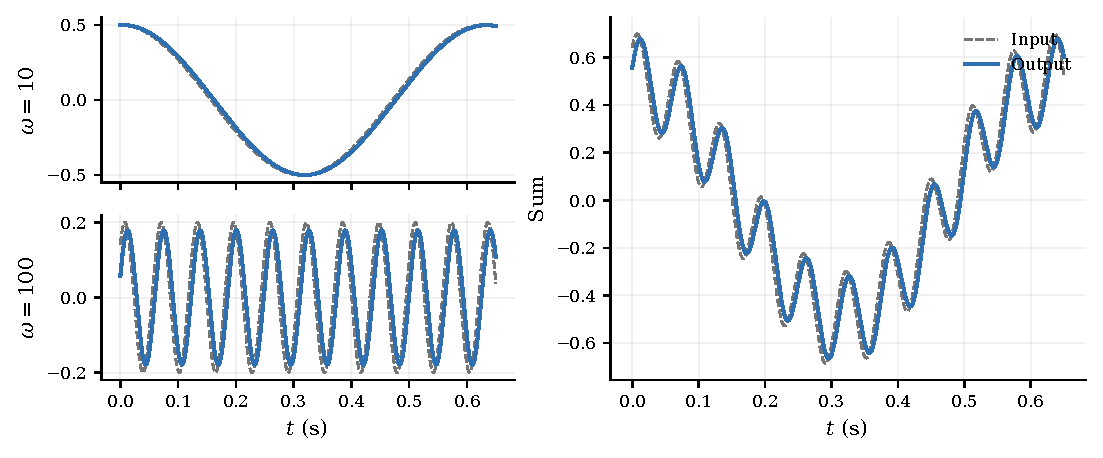
\includegraphics[width=.98\linewidth]{ch3-hw01-response.pdf}
\end{center}
左图分别比较低、高频分量，右图比较叠加波形；输入与输出曲线均为稳态表达式。高频分量衰减更明显，相位滞后也更大。

\textbf{为什么整体波形改变？}相对幅值由 $0.2/0.5=0.4$ 变为
$0.178885/0.499376\approx0.3582$，已经不满足共同幅值比。两成分的等效相位延迟分别为
\[
t_1=\frac{\arctan0.05}{10}\approx4.996\,\mathrm{ms},\qquad
t_2=\frac{\arctan0.5}{100}\approx4.636\,\mathrm{ms},
\]
也不完全相等。因此此输出不能严格写成 $A_0x(t-t_0)$。

\nt{\textbf{易错：}第二项的输出总相位是 $-71.5651^\circ$，系统新增相位差才是 $-26.5651^\circ$。若题目要求从 $t=0$ 接入信号后的全过程，还应按初始条件补上 $Ce^{-t/0.005}$；本题求稳态，不需保留该暂态项。}

\Needspace{8cm}
\subsection{例题2：由振幅误差确定时间常数}
\keypoint{复习重点：用最高频率约束 $\tau$；再将设计边界代入另一测量频率。}

\qs{100 Hz与50 Hz正弦测量}{用一阶系统测量 $100\,\mathrm{Hz}$ 正弦信号，要求振幅误差在 $5\%$ 以内，时间常数应取多少？若用该系统测量 $50\,\mathrm{Hz}$ 正弦信号，其振幅误差与相角差是多少？写出频响与稳态输出表达式。}

\sol
\textbf{先按静态灵敏度归一化。}取 $H(s)=1/(1+\tau s)$；若实际静态增益为 $K$，应先按 $K$ 标定后再计算动态相对误差。令
\[
\omega_{100}=2\pi\times100=200\pi\,\mathrm{rad/s}.
\]
一阶装置的幅值比小于等于1，故要求
\[
e_A=1-\frac{1}{\sqrt{1+(200\pi\tau)^2}}\leq0.05.
\]
整理不等式：
\begin{align*}
\frac{1}{\sqrt{1+(200\pi\tau)^2}}&\geq0.95,\\
(200\pi\tau)^2&\leq\frac{1}{0.95^2}-1,\\
\tau&\leq\frac{\sqrt{0.95^{-2}-1}}{200\pi}.
\end{align*}
因此，
\[
\boxed{0<\tau\leq5.23117\times10^{-4}\,\mathrm{s}
=0.523117\,\mathrm{ms}}.
\]
为得到具体的后续计算，取满足要求的\textbf{最大时间常数}
$\tau_{\max}=5.23117\times10^{-4}\,\mathrm{s}$。该边界设计的频响为
\[
\boxed{H(\iu\omega)=\frac{1}{1+\iu(5.23117\times10^{-4})\omega}},
\]
或写成 $H(\iu2\pi f)=1/[1+\iu2\pi f(5.23117\times10^{-4})]$。

在 $50\,\mathrm{Hz}$ 时，$\omega_{50}=100\pi\,\mathrm{rad/s}$，有
\[
q_{50}=\omega_{50}\tau_{\max}
=\frac12\sqrt{0.95^{-2}-1}=0.164342.
\]
因此
\begin{align*}
A_{50}&=\frac{1}{\sqrt{1+0.164342^2}}=0.986763,\\
e_{A,50}&=1-A_{50}=0.0132366
=\boxed{1.3237\%},\\
\phi_{50}&=-\arctan0.164342
=-0.162886\,\mathrm{rad}=\boxed{-9.3327^\circ}.
\end{align*}
若输入为 $x(t)=X_0\cos(100\pi t+\theta)$，则
\[
\boxed{y_{\mathrm{ss}}(t)=0.986763X_0
\cos(100\pi t+\theta-9.3327^\circ)}.
\]
输入若用正弦表示，则将余弦换成正弦，幅值比与相位差均不变。

\begin{table}[H]
\centering
\begin{tabular}{@{}c c c c@{}}
\toprule
频率 & $\omega\tau_{\max}$ & 振幅误差 & 相角差 \\
\midrule
$100\,\mathrm{Hz}$ & $0.328684$ & $5.0000\%$ & $-18.1949^\circ$ \\
$50\,\mathrm{Hz}$ & $0.164342$ & $1.3237\%$ & $-9.3327^\circ$ \\
\bottomrule
\end{tabular}
\end{table}

\nt{\textbf{易错：}本题频率单位是Hz，须先乘 $2\pi$；误差以理想输入幅值为基准，应令 $A\geq0.95$，不能写成 $A\geq1/1.05$。$50\,\mathrm{Hz}$ 的数值对应 $\tau=\tau_{\max}$；若取更小的 $\tau$，幅值误差和滞后角也更小。转折频率约为 $304.24\,\mathrm{Hz}$，但在转折点幅值已衰减约 $29.3\%$，不能把它当作5\%误差的测量上限。}

\Needspace{8cm}
\subsection{例题3：二阶装置阻尼比的选择}
\keypoint{复习重点：围绕幅值平坦、共振过载、相位线性和振铃抑制解释取值。}

\qs{为什么常用 $\zeta=0.6\sim0.8$}{试说明二阶测试装置阻尼比多采用 $0.6\sim0.8$ 的原因。}

\sol
阻尼比的选择需要兼顾幅值误差、共振过载、相位特性与瞬态响应。取 $K=1$，有
\[
A(r)=\frac{1}{\sqrt{1+(4\zeta^2-2)r^2+r^4}},\qquad
\phi(r)=-\operatorname{atan2}(2\zeta r,1-r^2).
\]

\textbf{第一，避免小阻尼造成明显共振放大。}
若 $0<\zeta<1/\sqrt2$，峰高为
$A_{\max}=1/[2\zeta\sqrt{1-\zeta^2}]$。例如
\[
\begin{array}{c|ccc}
\zeta & 0.14 & 0.6 & 0.7\\\hline
A_{\max} & 3.6070 & 1.0417 & 1.0002
\end{array}
\]
小阻尼 $0.14$ 可把固有频率附近的成分放大数倍；采用 $0.6\sim0.8$ 时峰值很小或不再出现，能降低共振附近干扰造成过载的风险。

\textbf{第二，低频幅值接近静态标定值。}
$\zeta\approx1/\sqrt2$ 时 $4\zeta^2-2\approx0$，幅值误差的低频二次项较小。阻尼过低使幅值上拱，阻尼过高使衰减更早出现；中间区间有利于保持一定宽度的近似平坦频带。

\textbf{第三，在低频工作区相位近似线性。}
当 $r\ll1$ 时，
\[
\phi(\omega)\approx-\frac{2\zeta}{\omega_n}\omega,
\]
对应共同延迟 $t_0\approx2\zeta/\omega_n$。配合足够高的固有频率，可使低频各成分接近同一延迟；它并不意味着相位差接近零。

\textbf{第四，抑制瞬态超调和振铃。}
欠阻尼阶跃超调 $M_p=e^{-\pi\zeta/\sqrt{1-\zeta^2}}$，在
$\zeta=0.6,0.7,0.8$ 时分别约为 $9.48\%$、$4.60\%$、$1.52\%$，明显小于很低阻尼时的超调。

\nt{\textbf{易错：}$0.6\sim0.8$ 是常用折中区间，不是任意频率下的精度保证；$\zeta=0.7$ 仍有极小的共振峰，不能笼统说“该区间全部无共振”。没有幅频共振峰的条件是 $\zeta\geq1/\sqrt2$，临界阻尼的条件是 $\zeta=1$。}

\Needspace{8cm}
\subsection{例题4：力传感器的幅值比与相角差}
\keypoint{复习重点：固有频率与测量频率用相同单位取比，比较阻尼改变后的幅值与相位。}

\qs{400 Hz正弦力通过二阶传感器}{某力传感器可作为二阶振荡系统处理，固有频率 $f_n=800\,\mathrm{Hz}$，阻尼比 $\zeta=0.14$。测量 $f=400\,\mathrm{Hz}$ 正弦力时，幅值比 $A(\omega)$ 与相角差 $\phi(\omega)$ 各为多少？若阻尼比改为 $0.7$，它们如何变化？}

\sol
\textbf{先把输出按静态灵敏度标定。}以下采用归一化模型 $K=1$，此时 $A$ 表示相对静态标定值的幅值比。频率比为
\[
r=\frac{\omega}{\omega_n}=\frac{2\pi f}{2\pi f_n}
=\frac{400}{800}=0.5,
\]
故 $1-r^2=0.75$。通用计算式为
\[
A=\frac{1}{\sqrt{0.75^2+(2\zeta\times0.5)^2}},\qquad
\phi=-\operatorname{atan2}(2\zeta\times0.5,0.75).
\]

\subsubsection{原装置：$\zeta=0.14$}
\[
H(\iu\omega)=\frac{1}{0.75+\iu0.14},
\]
\[
\boxed{A=\frac{1}{\sqrt{0.5625+0.0196}}=1.310694},\qquad
\boxed{\phi=-\arctan\frac{0.14}{0.75}=-10.5735^\circ}.
\]
静态标定后的幅值\textbf{高估约 $31.07\%$}，相位滞后约 $10.57^\circ$。
若输入 $F(t)=F_0\cos(800\pi t+\theta)$，归一化输出为
\[
z_{\mathrm{ss}}(t)=1.310694F_0\cos(800\pi t+\theta-10.5735^\circ).
\]

\subsubsection{增大阻尼：$\zeta=0.7$}
\[
H(\iu\omega)=\frac{1}{0.75+\iu0.7},
\]
\[
\boxed{A=\frac{1}{\sqrt{0.5625+0.49}}=0.974740},\qquad
\boxed{\phi=-\arctan\frac{0.7}{0.75}=-43.0251^\circ}.
\]
此时幅值\textbf{低估约 $2.526\%$}，但相位滞后增至约 $43.03^\circ$。归一化稳态输出为
\[
z_{\mathrm{ss}}(t)=0.974740F_0\cos(800\pi t+\theta-43.0251^\circ).
\]
若实际输出灵敏度为 $K$，上述输出幅值均再乘 $K$，相位不变。

\begin{center}
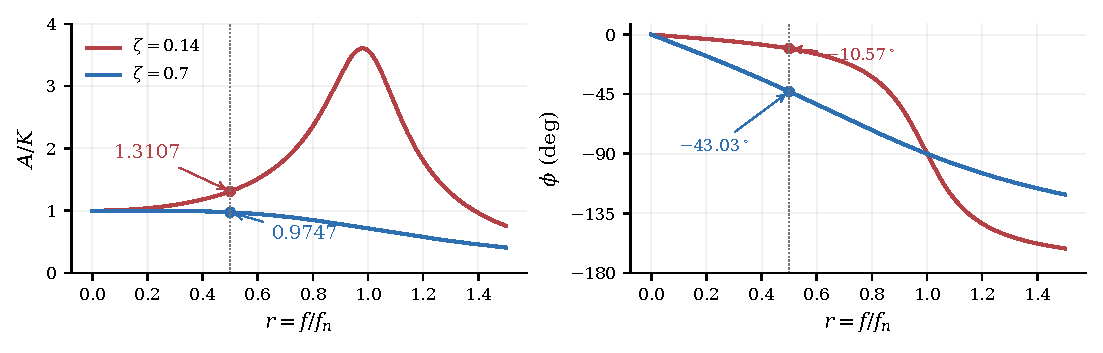
\includegraphics[width=.98\linewidth]{ch3-hw04-damping.pdf}
\end{center}
两条曲线都在 $r=0.5$ 处标出本题结果。对 $\zeta=0.14$，真正的幅频峰在 $r_r\approx0.9802$，峰高约为 $3.607$；测量点 $r=0.5$ 已有明显放大，但不是共振峰。

\begin{table}[H]
\centering
\begin{tabular}{@{}c c c c@{}}
\toprule
阻尼比 & 归一化幅值比 & 有符号幅值偏差 $A-1$ & 相角差 \\
\midrule
$0.14$ & $1.310694$ & $+31.0694\%$ & $-10.5735^\circ$ \\
$0.7$ & $0.974740$ & $-2.5260\%$ & $-43.0251^\circ$ \\
\bottomrule
\end{tabular}
\end{table}

\textbf{对阻尼选择的解释：}提高阻尼使 $400\,\mathrm{Hz}$ 处幅值更接近1，同时显著压低共振峰，支持适度阻尼的设计思路。但此测量点的相位滞后增大，因此不能概括为“阻尼增大，所有误差都减小”。若需要多频波形或同步测量，还必须检查相位条件。

\nt{\textbf{易错：}$800\,\mathrm{Hz}$ 是 $f_n$，不是 $\omega_n$；本题因频率取比，$2\pi$ 正好抵消。二阶幅值可能大于1，误差大小应取 $|A-1|$。单频相角差不是严格的波形失真判据，是否接受还取决于测量目标。}
